\chapter{Specifikacija programske potpore}
		
	\section{Funkcionalni zahtjevi}
			
			
			\noindent \textbf{Dionici:}
			
			\begin{packed_enum}
				
				\item Vlasnik sustava
				\item Glavni administrator konferencije				
				\item Operativni administrator
				\item Sudionik konferencije
				\item Razvojni tim
				\item Baza podataka
                \item Cloudinary
                \item Poslužitelj za vremensku prognozu
				
			\end{packed_enum}
			
			\noindent \textbf{Aktori i njihovi funkcionalni zahtjevi:}
			
			
			\begin{packed_enum}
				\item  \underbar{Neprijavljeni korisnik može:}
				
				\begin{packed_enum}
					
					\item pregledati aktivne konferencije i temeljne podatka o svakoj od tih konferencija
					
				\end{packed_enum}
			
				\item  \underbar{Vlasnik sustava može:}
				
				\begin{packed_enum}
    
                        \item Prijaviti se u sustav					
					\item Dodati konferenciju
					\item Kreirati korisnički račun glavnog admina svake konferencije
					
				\end{packed_enum}
				
				\item  \underbar{Glavni administrator može:}
				
				\begin{packed_enum}

                        \item Prijaviti se u sustav	
					\item Unijeti grupe podataka za konferenciju
					\item Kreirati korisničke račune za operativne admine konferencije
					\item Spremiti podatke o konferenciji nakon njenog završetka u obliku PDFa
					\item Postaviti multimedijske materijale sa konferencije i skinuti ih
					\item Pregledati sudionike konferencije po ulozi i državi iz koje dolaze
                        \item Kreirati poseban događaj i po potrebi povećati kapacitet
                        \item Pregledati detaljne podatke o svojoj konferenciji
					
				\end{packed_enum}
				
				\item  \underbar{Operativni administrator može:}
				
				\begin{packed_enum}

                         \item Prijaviti se u sustav	
					\item Kreirati korisničke račune sudionika konferencije
                        \item Pregledati detaljne podatke o svojoj konferenciji
					
				\end{packed_enum}
				
				\item  \underbar{Sudionik konferencije može:}
				
				\begin{packed_enum}

                        
					\item Prijaviti se u sustav
					\item Pregledati multimedijske materijale i skinuti ih
					\item Prijaviti se na posebna događanja
					\item Skinuti PDF potvrdu o sudjelovanju
                        \item Pregledati detaljne podatke o svojoj konferenciji
					
				\end{packed_enum}
				
				\item  \underbar{Baza podataka može:}
				
				\begin{packed_enum}
					
					\item Pohranjivati podatke o konferencijama
					\item Pohranjivati podatke o registriranim korisnicima
                        \item Pohranjivati podatke o posebnim događajima
                        \item Pohranjivati podatke o multimediji
                        \item Pohranjivati podatke o grupama podataka
					
				\end{packed_enum}
			\end{packed_enum}
			
			\eject 
			
			
				
			\subsection{Obrasci uporabe}
				
				
				\subsubsection{Opis obrazaca uporabe}
			
									\noindent \underbar{\textbf{UC1 -Pregled aktivnih konferencija}}
					\begin{packed_item}

                            
						\item \textbf{Glavni sudionik: }neprijavljeni korisnik, prijavljeni korisnik(sudionik, glavni admin, vlasnik sustava, operativni admin)
						\item  \textbf{Cilj:} Pregledati aktivne konferencije
						\item  \textbf{Sudionici:} Baza podataka
						\item  \textbf{Preduvjet:} -
						\item  \textbf{Opis osnovnog tijeka:}
						
						\item[] \begin{packed_enum}
	
							\item Popis konferencija vidljiv je odmah nakon pokretanja aplikacije
							\item Prikazuju se osnovne informacije o konferenciji: grad održavanja, opis konferencije i teme
						\end{packed_enum}
					\end{packed_item}

     \noindent \underbar{\textbf{UC2 - Registracija glavnog admina}}
					\begin{packed_item}
	
						\item \textbf{Glavni sudionik: }vlasnik sustava
						\item  \textbf{Cilj:} Stvoriti korisnički račun za  glavnog admina konferencije
						\item  \textbf{Sudionici:} Baza podatka, glavni admin
						\item  \textbf{Preduvjet:} -
						\item  \textbf{Opis osnovnog tijeka:}
						
						\item[] \begin{packed_enum}

							\item Vlasnik sustava odabere opciju \textit{Registriraj}
							\item Vlasnik sustava unosi potrebne podatke: ime, prezime, broj telefona, e-mail, adresu, državu, naziv poduzeća iz koje dolazi, svojstvo sudjelovanja na konferenciji
                                \item Povratak na meni
						
						\end{packed_enum}
						\item  \textbf{Opis mogućih odstupanja:}
						
						\item[] \begin{packed_item}

                                    \item[1.]  Unos već zauzetog korisničkog imena, unos podataka u nedozvoljenom       formatu ili pružanje neispravnog e-maila:
							\item[] \begin{packed_enum}
								
								\item Sustav obavještava glavnog sudionika o neuspjelom upisu
								\item Glavni sudionik mijenja potrebne podatke te završava unos ili odustaje od registracije
							
						\end{packed_enum}
					\end{packed_item}
     \end{packed_item}

     				 \noindent \underbar{\textbf{UC3 - Registracija operativnog admina}}
					\begin{packed_item}
	
						\item \textbf{Glavni sudionik: }glavni admin
						\item  \textbf{Cilj:} Stvoriti korisnički račun za  operativnog admina konferencije
						\item  \textbf{Sudionici:} Baza podatka, operativni admin
						\item  \textbf{Preduvjet:} -
						\item  \textbf{Opis osnovnog tijeka:}
						
						\item[] \begin{packed_enum}

							\item Glavni admin odabere opciju \textit{Registriraj}
							\item Glavni admin unosi potrebne podatke: ime, prezime, broj telefona, e-mail, adresu, državu, naziv poduzeća iz koje dolazi, svojstvo sudjelovanja na konferenciji
                                \item Povratak na meni
						
						\end{packed_enum}
						\item  \textbf{Opis mogućih odstupanja:}
						
						\item[] \begin{packed_item}

                                    \item[1.]  Unos već zauzetog korisničkog imena, unos podataka u nedozvoljenom       formatu ili pružanje neispravnog e-maila:
							\item[] \begin{packed_enum}
								
								\item Sustav obavještava glavnog sudionika o neuspjelom upisu
								\item Glavni sudionik mijenja potrebne podatke te završava unos ili odustaje od registracije
							
						\end{packed_enum}
					\end{packed_item}
     \end{packed_item}

      \noindent \underbar{\textbf{UC4 - Registracija sudionika}}
					\begin{packed_item}
	
						\item \textbf{Glavni sudionik: }operativni admin
						\item  \textbf{Cilj:} Stvoriti korisnički račun za  sudionika konferencije
						\item  \textbf{Sudionici:} Baza podatka, operativni admin
						\item  \textbf{Preduvjet:} Plaćena kotizacija
						\item  \textbf{Opis osnovnog tijeka:}
						
						\item[] \begin{packed_enum}

							\item Operativni admin odabere opciju \textit{Registriraj}
							\item Operativni admin unosi potrebne podatke: ime, prezime, broj telefona, e-mail, adresu, državu, naziv poduzeća iz koje dolazi, svojstvo sudjelovanja na konferenciji
                                \item Sustav šalje mail s linkom za potvrdu registracije sudioniku
                                \item Povratak na meni
						
						\end{packed_enum}
						\item  \textbf{Opis mogućih odstupanja:}
						
						\item[] \begin{packed_item}

                                \item[1.]  Sudionik nije platio kotizaciju
							\item[] \begin{packed_enum}
								
								\item Odustaje se od registracije

                                    \item[2.]  Unos već zauzetog korisničkog imena, unos podataka u nedozvoljenom       formatu ili pružanje neispravnog e-maila:
							\item[] \begin{packed_enum}
								
								\item Sustav obavještava glavnog sudionika o neuspjelom upisu
								\item Glavni sudionik mijenja potrebne podatke te završava unos ili odustaje od registracije
							
						\end{packed_enum}
                    \end{packed_enum}
					\end{packed_item}
     \end{packed_item}

     \noindent \underbar{\textbf{UC5 - Prijava u sustav}}
					\begin{packed_item}
	
						\item \textbf{Glavni sudionik: } Korisnik
						\item  \textbf{Cilj:} Dobiti pristup korisničkom sučelju
						\item  \textbf{Sudionici:} Baza podataka
						\item  \textbf{Preduvjet:} Registracija uspješna
						\item  \textbf{Opis osnovnog tijeka:}
						
						\item[] \begin{packed_enum}
	
							\item Korisnik odabere opciju \textit{Prijavi se}
							\item Korisnik unosi korisničko ime i lozinku
							\item Pristup korisničkim funkcijama
						\end{packed_enum}
						
						\item  \textbf{Opis mogućih odstupanja:}
						
						\item[] \begin{packed_item}
	
							\item[1.] Neispravno korisničko ime i lozinka

							\item[] \begin{packed_enum}
								
								\item Sustav obavještava korisnika o neuspjeloj prijavi porukom "Login failed"
								
							\end{packed_enum}
							
						\end{packed_item}
					\end{packed_item}

     \noindent \underbar{\textbf{UC6 - Stvaranje konferencije}}
					\begin{packed_item}
	
						\item \textbf{Glavni sudionik: } vlasnik sustava
						\item  \textbf{Cilj:} Unijeti temeljne podatke o konferenciji u sustav
						\item  \textbf{Sudionici:} Baza podataka
						\item  \textbf{Preduvjet:} -
						\item  \textbf{Opis osnovnog tijeka:}
						
						\item[] \begin{packed_enum}
	
							\item Vlasnik sustava odabere opciju \textit{Dodaj konferenciju}
							\item Vlasnik unosi temeljne podatke: naziv, mjesto i vrijeme, teme, događaji, glavnog administratora konferencije
							\item Konferencija se prikazuje u sustavu
						\end{packed_enum}

                        \item  \textbf{Opis mogućih odstupanja:}
						
						\item[] \begin{packed_item}
	
							\item[1.] Nisu uneseni svi podatci

							\item[] \begin{packed_enum}
								
								\item Sustav obavještava korisnika da mora unijeti sve podatke za konferenciju
								
							\end{packed_enum}
							
						\end{packed_item}
						
					\end{packed_item}


     					\noindent \underbar{\textbf{UC7 - Unos grupa podataka za konferenciju}}
					\begin{packed_item}
	
						\item \textbf{Glavni sudionik: } glavni administrator
						\item  \textbf{Cilj:} unijeti grupe podataka za konferenciju
						\item  \textbf{Sudionici:} baza podataka
						\item  \textbf{Preduvjet:} konferencija stvorena
						\item  \textbf{Opis osnovnog tijeka:}
						
						\item[] \begin{packed_enum}

                                \item Glavni admin najprije unosi glavne grupe podataka
							\item Glavni admin odabere opciju \textit{Unos podataka}
							\item Glavni admin unosi do najviše 15 grupa podataka među kojima su obavezni: raspored predavanja, zbornik radova, prezentacije predavanja i mjesto događaja
							\item Detaljni podaci dostupni registriranim korisnicima na pregled
						\end{packed_enum}
						
						\item  \textbf{Opis mogućih odstupanja:}
						
						\item[] \begin{packed_item}
	
							\item[1.] Nepotpuno ispunjavanje obveznih grupa podataka
							\item[] \begin{packed_enum}
								
								\item Admin ne može unijeti ostale grupe podataka

                                    \end{packed_enum}
                                \item[2.] Nepotpuno ispunjavanje forme za kreiranje neobavezne grupe podataka
							\item[] \begin{packed_enum}
								
								\item Sustav obaviještava admina da mora unijeti sve podatke
                                \end{packed_enum}
        
                                \item[3.] Admin pokušava unijeti više od 15 grupa podataka
							\item[] \begin{packed_enum}
								
								\item Sustav obaviještava admina da ne može unijeti sve podatke

                                    \end{packed_enum}
							
						\end{packed_item}
					\end{packed_item}

     \noindent \underbar{\textbf{UC8 - Spremanje podataka o konferenciji u obliku PDF-a}}
					\begin{packed_item}
	
						\item \textbf{Glavni sudionik: }Glavni administrator

						\item  \textbf{Cilj:} spremiti sve podatke prije zaključenja rada s aplikacijom
						\item  \textbf{Sudionici:} baza podataka
						\item  \textbf{Preduvjet:} -
						\item  \textbf{Opis osnovnog tijeka:}
						
						\item[] \begin{packed_enum}
	
							\item Glavni admin odabire opciju \textit{Spremi konferenciju}
							\item Podaci se spremaju na lokalno računalo u obliku PDF-a
							
						\end{packed_enum}
						
						
						\end{packed_item}

     \noindent \underbar{\textbf{UC9 - Postavljanje multimedijskih sadržaja}}
					\begin{packed_item}
	
						\item \textbf{Glavni sudionik: }Glavni administrator

						\item  \textbf{Cilj:} ponuditi pregled i skidanje multimedijskog sadržaja registriranim korisnicima
						\item  \textbf{Sudionici:} poslužitelj Cloudinary
						\item  \textbf{Preduvjet:} -
						\item  \textbf{Opis osnovnog tijeka:}
						
						\item[] \begin{packed_enum}
	
							\item Glavni admin odabire opciju \textit{Dodaj multimedijski sadržaj}
							\item Glavni admin dodaje direktorij za pojedini dan ili odabire postojeći direktorij
                                \item Glavni admin postavlja multimedijski sadržaj za pojedini dan
							
						\end{packed_enum}
                     \item  \textbf{Opis mogućih odstupanja:}
						
						\item[] \begin{packed_item}
	
							\item[1.] Pokušava se kreirati direktorij s datumom koji nije unutar datuma održavanja konferencije

							\item[] \begin{packed_enum}
								
								\item Sustav obavještava korisnika da uneseni datum nije dobar
								
							\end{packed_enum}
							
						\end{packed_item}
										
						\end{packed_item}

     \noindent \underbar{\textbf{UC10 - Pregled sudionika konferencije}}
					\begin{packed_item}
	
						\item \textbf{Glavni sudionik: }Glavni administrator

						\item  \textbf{Cilj:} Pregled prijavljenih sudionika
						\item  \textbf{Sudionici:} Baza podataka
						\item  \textbf{Preduvjet:} -
						\item  \textbf{Opis osnovnog tijeka:}
						
						\item[] \begin{packed_enum}
	
							\item Glavni admin odabere opciju \textit {Pregled prijavljenih sudionika}
							\item Prikazuju se podaci o prijavljenim sudionicima (status i država iz koje dolaze)
							
						\end{packed_enum}
						
						
						\end{packed_item}
				
						\noindent \underbar{\textbf{UC11 - Pregled multimedijskih sadržaja}}
					\begin{packed_item}
						
						\item \textbf{Glavni sudionik:} Korisnik(sudionik, glavni admin ili operativni admin)
						\item  \textbf{Cilj:} Pregled multimedijskih materijala po danima i mogućnost preuzimanja na lokalno računalo
						\item  \textbf{Sudionici:} Poslužitelj Cloudinary
						\item  \textbf{Preduvjet:} Glavni administrator konferencije je postavio multimedijske materijale na poslužitelj
						\item  \textbf{Opis osnovnog tijeka:}
						
						\item[] \begin{packed_enum}
							
							\item Korisnik odabere opciju \textit{Pregled multimedijskog sadržaja}
							\item Korisniku se prikazuju multimedijski materijali po danima
							\item Korisnik ih može preuzeti klikom na gumb "Preuzmi"
						\end{packed_enum}
					\end{packed_item}

			
						\noindent \underbar{\textbf{UC12 - Prijava na poseban događaj}}
					\begin{packed_item}
						
						\item \textbf{Glavni sudionik:} Sudionik konferencije
						\item  \textbf{Cilj:} Prijava na posebni događaj
						\item  \textbf{Sudionici:} Baza podataka
						\item  \textbf{Preduvjet:} -
						\item  \textbf{Opis osnovnog tijeka:}
						
						\item[] \begin{packed_enum}
							
							\item Korisnik odabere opciju \textit{Prijavi se na posebni događaj}
							\item Sustav ispisuje potvrdu o uspješnoj prijavi
						\end{packed_enum}
						\item  \textbf{Opis mogućih odstupanja:}
					
					\item[] \begin{packed_item}
						
						\item[1.] Sva mjesta za željeni događaj su zauzeta
						\item[] \begin{packed_enum}

                                \item Sudionik se stavlja u listu čekanja za događaj
							\item Sustav obavještava glavnog administratora o prekobrojnoj potražnji za već popunjeni događaj i mogućnosti povećanja broja sudionika
							
						\end{packed_enum}
						
					\end{packed_item}
				\end{packed_item}
			
				\noindent \underbar{\textbf{UC13 - Generiranje PDF potvrde o sudjelovanju}}
			\begin{packed_item}
				
				\item \textbf{Glavni sudionik:} Korisnik
				\item  \textbf{Cilj:} Generiranje PDF potvrde
				\item  \textbf{Sudionici:} baza podataka
				\item  \textbf{Preduvjet:} -
				\item  \textbf{Opis osnovnog tijeka:}
				
				\item[] \begin{packed_enum}
					
					\item Korisnik bira opciju \textit{Potvrda o sudjelovanju}
					\item Sustav generira PDF dokument o sudjelovanju
					\item Korisnik može preuzeti pdf potvrdu
				\end{packed_enum}
			\end{packed_item}

        \noindent \underbar{\textbf{UC14 - Povećanje kapaciteta posebnog događaja}}
			\begin{packed_item}
				
				\item \textbf{Glavni sudionik:} Glavni admin
				\item  \textbf{Cilj:} Povećanje kapaciteta posebnog događaja
				\item  \textbf{Sudionici:} baza podataka
				\item  \textbf{Preduvjet:} Popunjenost kapaciteta posebnog događaja, postoji poseban događaj
				\item  \textbf{Opis osnovnog tijeka:}
				
				\item[] \begin{packed_enum}
					
					\item Glavni admin bira opciju \textit{Povećaj kapacitet}
					\item Sustav ažurira broj mjesta na posebnom događaju
					\item Sudionik koji je bio u listi čekanja dobiva mail obavijest da se mjesto otvorilo
				\end{packed_enum}
			\end{packed_item}

    \noindent \underbar{\textbf{UC15 - Stvaranje posebnog događaja}}
			\begin{packed_item}
				
				\item \textbf{Glavni sudionik:} Glavni admin
				\item  \textbf{Cilj:} Stvoriti poseban događaj na konferenciji
				\item  \textbf{Sudionici:} baza podataka
				\item  \textbf{Preduvjet:} -
				\item  \textbf{Opis osnovnog tijeka:}
				
				\item[] \begin{packed_enum}
					
					\item Glavni admin bira opciju \textit{Kreiraj posebni događaj}
					\item Glavni admin unosi kapacitet, tip posebnog događaja i poruku sudionicima
					\item Poseban događaj se dodaje kao grupa podataka konferencije
				\end{packed_enum}
         \item  \textbf{Opis mogućih odstupanja:}
					
					\item[] \begin{packed_item}
						
						\item[1.] Nisu uneseni svi podatci
						\item[] \begin{packed_enum}

                                \item Sustav obaviještava korisnika da mora unijeti sve podatke
							
						\end{packed_enum}
						
					\end{packed_item}
			\end{packed_item}



   \noindent \underbar{\textbf{UC16 - Pregled podataka o konferenciji}}
			\begin{packed_item}
				
				\item \textbf{Glavni sudionik:} Registrirani korisnik
				\item  \textbf{Cilj:} Pregledati detaljne podatke o konferenciji
				\item  \textbf{Sudionici:} baza podataka, poslužitelj za vremensku prognozu
				\item  \textbf{Preduvjet:} -
				\item  \textbf{Opis osnovnog tijeka:}
				
				\item[] \begin{packed_enum}
					
					\item Korisnik bira opciju \textit{ Moja konferencija }
					\item Prikazuje se stranica sa svim podacima o konferenciji
         
					\end{packed_item}
			\end{packed_item}
	
     
					
				\subsubsection{Dijagrami obrazaca uporabe}
					
						\begin{figure}[H]
			            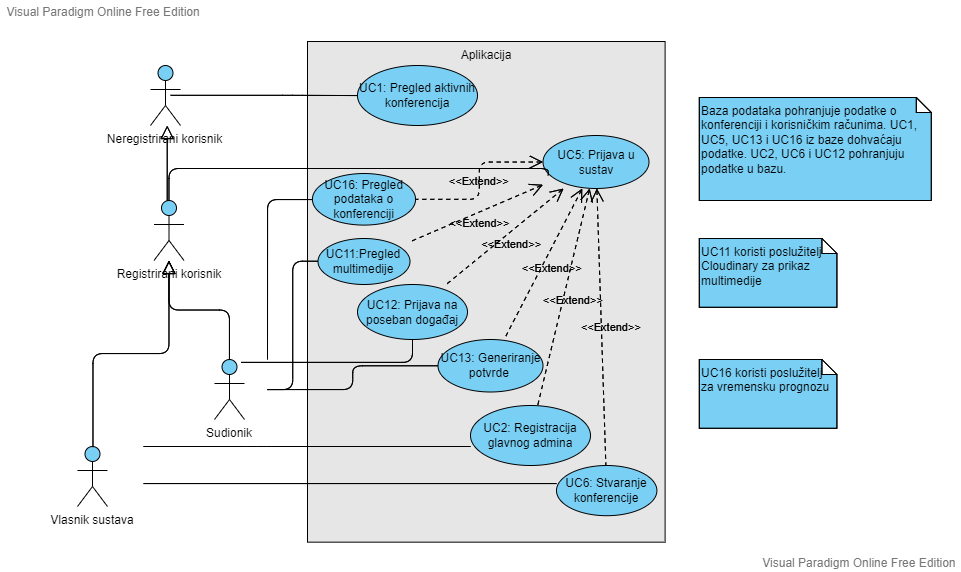
\includegraphics[scale=0.5]{slike/UC_diagram_1.png} %veličina slike u odnosu na originalnu datoteku i pozicija slike
			            \centering
			            \caption{Funkcionalnosti za sudionika i vlasnika sustava}
			            \label{fig:uc-dijagram1}
		                \end{figure}
		                
		                \begin{figure}[H]
			            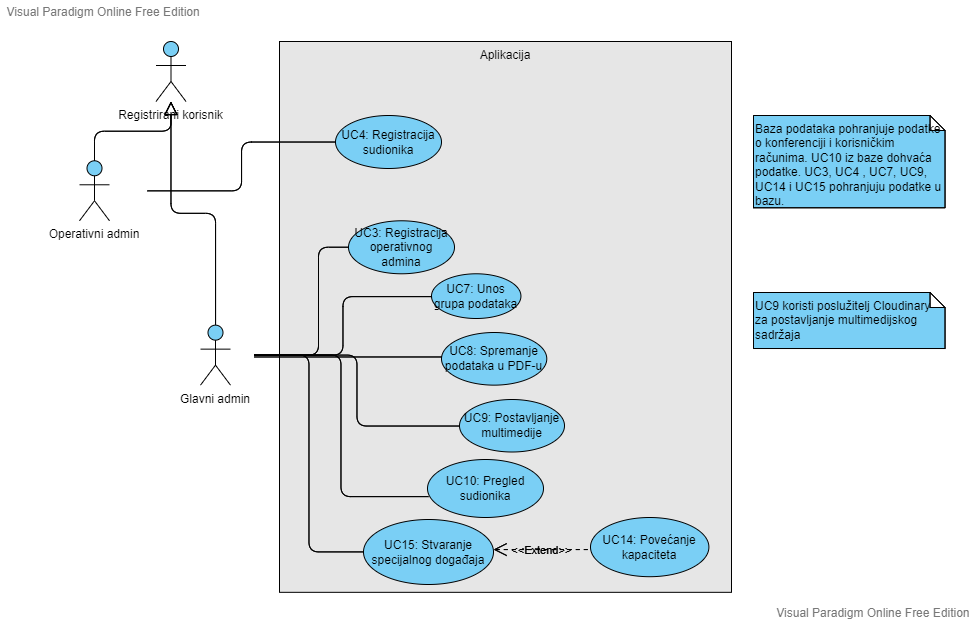
\includegraphics[scale=0.5]{slike/UC_diagram_2.png} %veličina slike u odnosu na originalnu datoteku i pozicija slike
			            \centering
			            \caption{Funkcionalnosti za glavnog admina i operativnog admina}
			            \label{fig:uc-dijagram2}
		                \end{figure}
				\eject		
				
			\subsection{Sekvencijski dijagrami}
				
	

            \textbf{UC7: Unos grupa podataka za konferenciju}\\
				
				{Glavni admin konferencije unosi grupe podataka za svoju konferenciju. Postoje 4 obavezne grupe podataka: raspored predavanja, zbornik radova, prezentacije predavanja i lokacija događanja te jedna grupa podataka koja je obavezna samo ako postoji posebni događaj - obavijest o posebnom događaju. Glavni admin mora prvo unijeti obavezne grupe podataka, a onda tek smije unijeti dodatne podatke. Moguće je unijeti maksimalno 15 grupa podataka za neku konferenciju. Ukoliko je već uneseno 15 grupa podataka aplikacija obaviještava admina porukom.}
				
		        \begin{figure}[H]
			            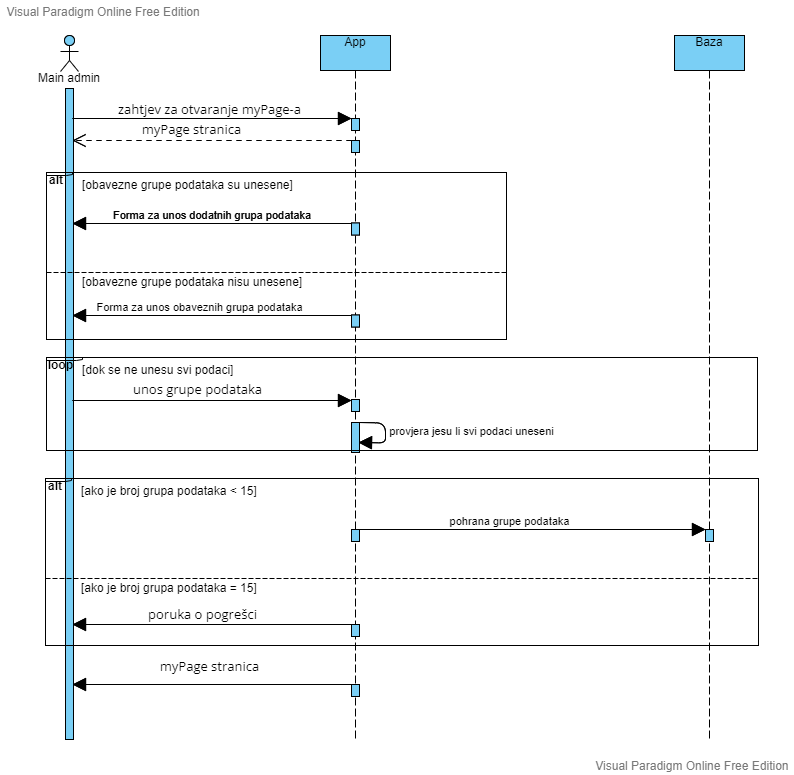
\includegraphics[scale=0.55]{slike/stvaranje grupe podataka (1).png} %veličina slike u odnosu na originalnu datoteku i pozicija slike
			            \centering
			            \caption{Unos grupe podataka}
			            \label{fig:seq-dijagram2}
		        \end{figure}\\
				
				\eject

             \textbf{UC15: Stvaranje posebnog događaja}\\
				
				{Glavni admin stvara posebna događanja za konferenciju. S obzirom da se stvaranjem posebnog događaja stvara i grupa podataka tj. obavijest, provjerava se je li dosegnut maksimalan broj grupa podataka. Ukoliko nije, stvara se posebni događaj i obavijest o tom posebnom događaju, u suprotnom se obaviještava admina o pogrešci.}
				
		        \begin{figure}[H]
			            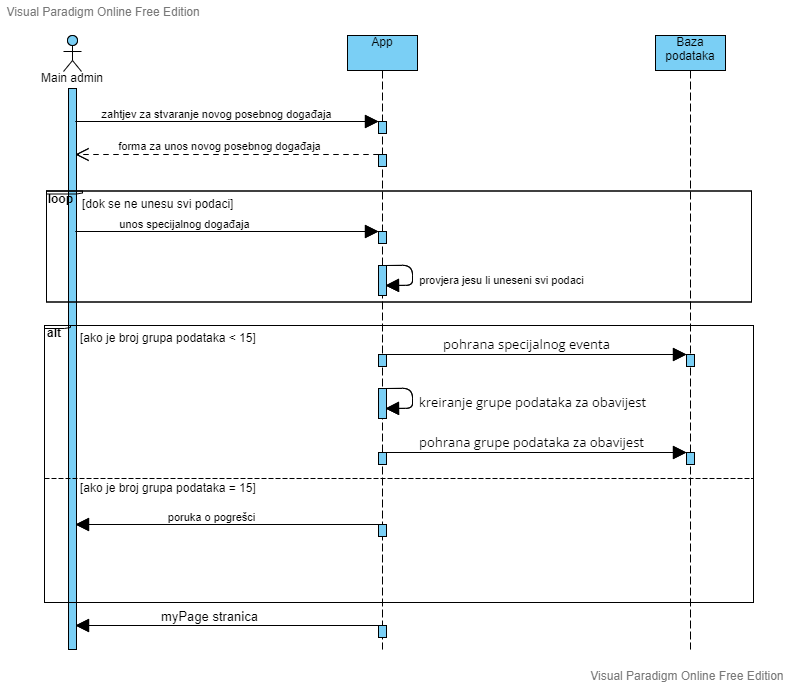
\includegraphics[scale=0.55]{slike/stvaranje spec eventa.png} %veličina slike u odnosu na originalnu datoteku i pozicija slike
			            \centering
			            \caption{Unos posebnog događaja}
			            \label{fig:seq-dijagram2}
		        \end{figure}\\
				
				\eject

             \textbf{UC5: Prijava u sustav, UC6: Stvaranje konferencije, UC2: Registracija glavnog admina}\\
				
				{Vlasnik sustava se prijavljuje u aplikaciju. Ako je prijava uspješna, vlasnik sustava dobiva pristup aplikaciji, inače dobiva poruku o neuspjeloj prijavi i može pokušati opet. Vlasnik sustava odabire opciju kreiranja konferencije i unosi glavne podatke o konferenciji. Ako nisu uneseni svi podatci, sustav to dojavljuje vlasniku. Ako je sve ispravno uneseno, stvara se nova konferencija i vlasnik sustava je preusmjeren na formu za registraciju glavnog admina te konferencije. Unosi podatke o glavnom adminu i pridružuje ga upravo napravljenoj konferenciji. Ako je sve ispravno uneseno, stvoren je račun glavnog admina i vlasnik sustava je preusmjeren na menu page, inače dobiva poruku o netočno unesenim podatcima.}
				
		        \begin{figure}[H]
			            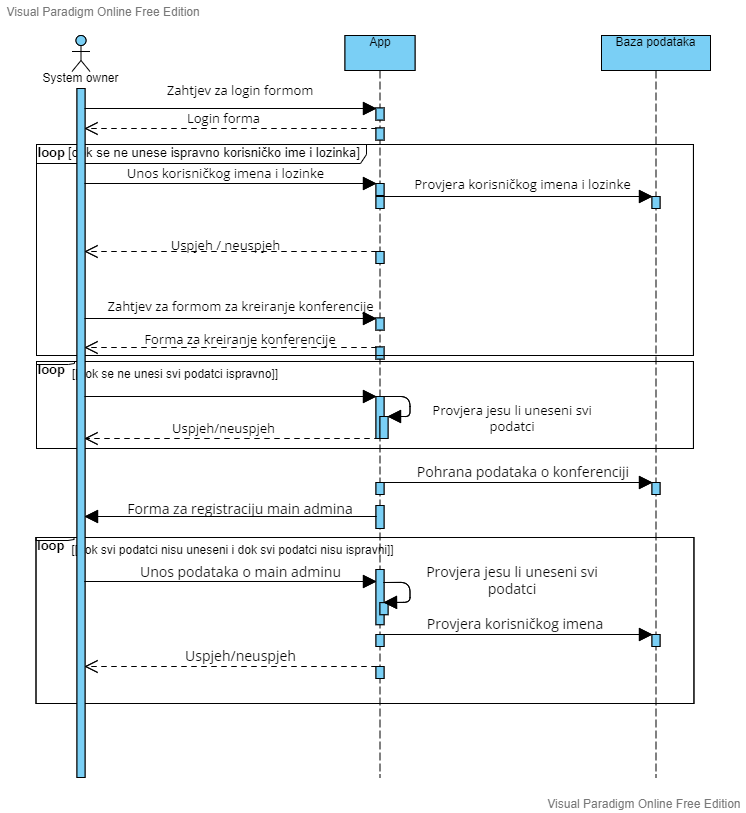
\includegraphics[scale=0.55]{slike/Stvaranje_konf_seq.png} %veličina slike u odnosu na originalnu datoteku i pozicija slike
			            \centering
			            \caption{Stvaranje konferencije i main admina konferencije}
			            \label{fig:seq-dijagram2}
		        \end{figure}\\
				
				\eject

             \textbf{UC12: Prijava na poseban događaj}\\
				
				{Sudionik konferencije odabire opciju prijave na poseban događaj. Ako ima još slobodnih mjesta, korisnik postaje sudionik tog posebnog događaja, a broj slobodnih mjesta se umanjuje za jedan. Ako nema slobodnih mjesta, sudionik se stavlja u listu čekanja, a sustav šalje mail obavijest glavnom adminu konferencije da su sva mjesta na specijalnom događaju popunjena. Nakon toga, glavni admin može povećati broj mjesta. Ako to učini, sustav šalje mail obavijest korisniku da je primljen na poseban događaj te ažurira broj slobodnih mjesta.}
				
		        \begin{figure}[H]
			            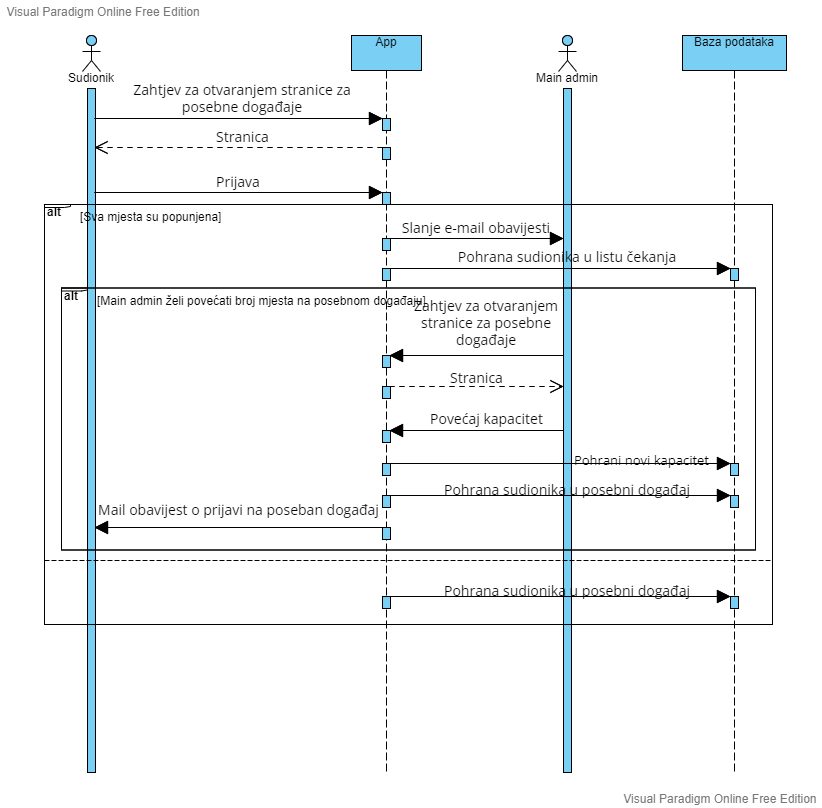
\includegraphics[scale=0.55]{slike/Spec_event_prijava_seq.png} %veličina slike u odnosu na originalnu datoteku i pozicija slike
			            \centering
			            \caption{Prijava na poseban događaj}
			            \label{fig:seq-dijagram2}
		        \end{figure}\\
	
				\eject
	
		\section{Nefunkcionalni zahtjevi}
		
		 
			\begin{packed_item}  
				 \item Sustav treba biti implementiran kao web aplikacija koristeći objektno-orijentirane jezike
				 \item Pristup sustavu mora biti omogućen iz javne mreže pomoću HTTPS
				 \item Sustav treba omogućiti rad više korisnika u stvarnom vremenu, preko 500
				 \item Sustav treba biti izdržljiv na neispravno korištenje
				 \item Izvršavanje dijela programa u kojem se pristupa bazi podataka ne smije trajati duže od nekoliko sekundi
				 \item Nadogradnja sustava ne smije narušavati postojeće funkcionalnosti sustava
				 \item Veza s bazom podataka mora biti zaštićena i otporna na vanjske greške
				 \item Učitavanje prikaza ne smije trajati duže od nekoliko sekundi
				 \item Pristup sustavu treba biti omogućen samo registriranim korisnicima i zaštićen od vanjskih sudionika
                \item Tokeni za potvrdu e-mail adrese traju 24 sata
                \item Tokeni za autentifikaciju traju 1 sat
                \item Korisničko sučelje i sustav moraju podržavati hrvatsku abecedu (dijakritičke znakove) pri unosu i prikažu tekstualnog sadrzaja
                \item Neispravno korištenje korisničkog sučelja ne smije narušiti funkcionalnost i rad sustava
                \item Korisnički podaci trebaju biti sigurno pohranjeni i odgovarajuće enkriptirani
                \item Korisničko sučelje treba biti jednostavno, intuitivno i pregledno, korisnici se moraju znati koristiti sučeljem bez opširnih uputa
                \item Korisnicima su podatci o njihovoj konferenciji dostupni do 30 dana nakon njenog završetka
                \item Glavni administrator do 40 dana nakon završetka konferencije može spremati podatke
                \item Glavnom administatoru zabranjeno je stvoranje specijalnog događaja ili grupe podataka za konferenciju koja već ima 15 grupa podataka

			\end{packed_item}
	